\section{Discrete Probability Distribution}

Suppose that a number is assigned to each point of the sample space. Then we have defined a \emph{function} on the sample space. This function is called a \emph{random variable} (or \emph{stochastic variable}) or more precisely a \emph{random function}.

Usually, random variables are denoted by capital letters such as $X$ or $Y$. In general, a random variable has some physical, geometric, economic, financial, or other meaning.

\begin{ejemplo}
	\label{exmp:2.6.1}
	Suppose that a coin is tossed twice so that the sample space is $\set{HH,HT,TH,TT}.$ Let $X$ represent the number of heads ($H$) obtained.
\end{ejemplo}

\subsection{Discrete Probability Mass Functions (PMF and Support)}
\subsubsection{Discrete Probability Functions}

Let $X$ be a discrete random variable. Suppose that the values it can take are $x_{1},...,x_{k},$ arranged in some given order. Suppose also that these values have some probability given by
\begin{align}
	\label{eq:2.6.1}
	P(X=x_{k})=f(x_{k}).
\end{align}

{Probability function}
\begin{align}
	\label{2.2}
	P(X=x)=
	\begin{cases}
		f(x) & x=x_{k} \\
		0	& \text{otherwise}
	\end{cases}
\end{align}

In general, $f(x)$ will be a probability function if
\begin{align}
	\begin{cases}
		f(x)\geq 0 \\
		\sum_{x}f(x)=1.
	\end{cases}
\end{align}

\begin{ejemplo}
	\label{exmp:2.6.2}
	Find the probability function corresponding to the random variable $X$ from Example \ref{exmp:2.6.1}.
\end{ejemplo}

\begin{solucion}
	The sample space is $\{HH, HT, TH, TT\}$, each with probability $\frac{1}{4}$.
	
	$X$ = number of heads ($H$):
	\begin{itemize}
		\item $X = 0$ for $TT$: $P(X=0) = \frac{1}{4}$
		\item $X = 1$ for $HT, TH$: $P(X=1) = \frac{2}{4} = \frac{1}{2}$
		\item $X = 2$ for $HH$: $P(X=2) = \frac{1}{4}$
	\end{itemize}
	
	The probability function is:
	\begin{align}
		f(x) = \begin{cases}
			\frac{1}{4} & x = 0 \\
			\frac{1}{2} & x = 1 \\
			\frac{1}{4} & x = 2 \\
			0 & \text{otherwise}
		\end{cases}
	\end{align}
\end{solucion}

\begin{ejemplo}
	\label{exmp:2.6.3}
	Suppose that a pair of dice is rolled. Let $X$ be the random variable given by the sum of the points. Find the probability distribution of $X.$
\end{ejemplo}

\begin{solucion}
	The sample space has $6 \times 6 = 36$ outcomes. The variable $X$ takes values from 2 to 12.
	
	\begin{align}
		f(x) = P(X=x) = \frac{\text{number of ways to obtain } x}{36}
	\end{align}
	
	\begin{center}
	\begin{tabular}{c|ccccccccccc}
		$x$ & 2 & 3 & 4 & 5 & 6 & 7 & 8 & 9 & 10 & 11 & 12 \\
		\hline
		$f(x)$ & $\frac{1}{36}$ & $\frac{2}{36}$ & $\frac{3}{36}$ & $\frac{4}{36}$ & $\frac{5}{36}$ & $\frac{6}{36}$ & $\frac{5}{36}$ & $\frac{4}{36}$ & $\frac{3}{36}$ & $\frac{2}{36}$ & $\frac{1}{36}$
	\end{tabular}
	\end{center}
\end{solucion}

\begin{ejemplo}
	\label{exmp:2.6.4}
	Find the probability distribution of boys and girls in families with 3 children, assuming equal probability for boys and girls.
\end{ejemplo}

\begin{solucion}
	Let $X$ = number of boys. Each child is a boy (B) or girl (G) with probability $\frac{1}{2}$.
	
	The sample space has $2^3 = 8$ outcomes: $\{BBB, BBG, BGB, BGG, GBB, GBG, GGB, GGG\}$.
	
	$X$ can take values 0, 1, 2, 3:
	\begin{align}
		f(x) = \begin{cases}
			\frac{1}{8} & x = 0 \text{ (GGG)} \\
			\frac{3}{8} & x = 1 \text{ (BGG, GBG, GGB)} \\
			\frac{3}{8} & x = 2 \text{ (BBG, BGB, GBB)} \\
			\frac{1}{8} & x = 3 \text{ (BBB)}
		\end{cases}
	\end{align}
	
	This is an example of a binomial distribution with $N=3$ and $p=\frac{1}{2}$.
\end{solucion}

\subsection{Cumulative Distribution Function for Discrete Random Variables (CDF)}

The distribution function of a discrete variable $X$ is obtained from the probability function via the following formula:
\begin{align}
	\label{eq:2.6.2}
	F(x) = P(X\leq x) = \sum_{u \leq x} f(u).
\end{align}

If $X$ takes only a finite number of values $x_{1},...,x_{n}$, then the distribution function is given by
\begin{align}
	\label{eq:2.6.3}
	F(x)=
	\begin{cases}
		0 & -\infty < x < 0 \\
		f(x_{1}) & x_{1} \leq x < x_{2} \\
		f(x_{1})+f(x_{2}) & x_{2} \leq x < x_{3} \\
		\vdots & \vdots \\
		f(x_{1})+\cdots+f(x_{n}) & x_{n} \leq x < \infty
	\end{cases}
\end{align}

\begin{ejemplo}
	\label{exmp:2.6.5}
	Find the distribution function for the random variable $X$ from Example \ref{exmp:2.6.2} and obtain its graph.
\end{ejemplo}

\begin{figure}
	\centering
	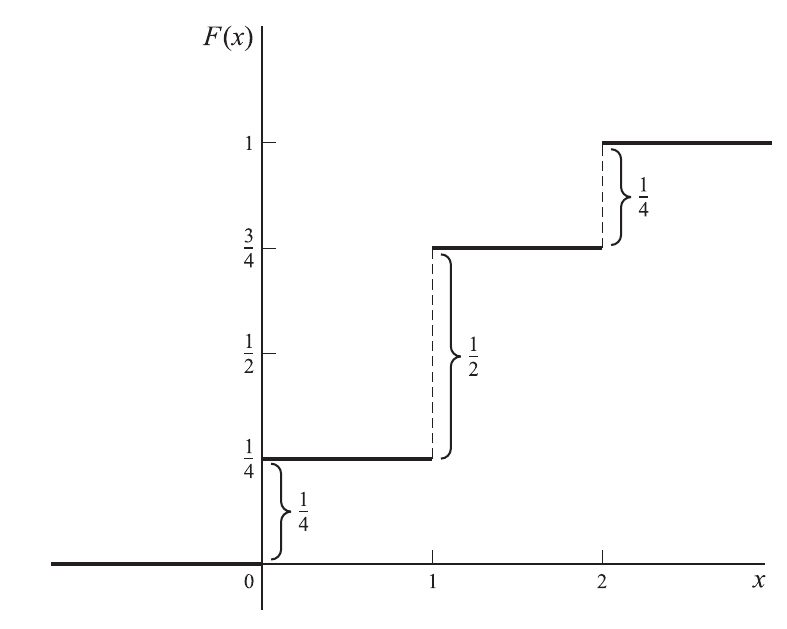
\includegraphics[height=7cm,keepaspectratio=true]{./pe/pands0201.png}
	% pands0201.png: 0x0 pixel, 300dpi, 0.00x0.00 cm, bb=
	\label{fig:2.6.1}
\end{figure}

\begin{observacion}
	\begin{itemize}
		\item The jumps in the distribution function are determined by the value of the probability function.
		\item This type of function is known as a \emph{step function}. Note that it is \emph{right-continuous.}
		\item The distribution function is \emph{monotonically increasing.}
	\end{itemize}
\end{observacion}

The probability function can be obtained from the distribution function via the following formula:
\begin{align}
	\label{eq:2.6.4}
	f(x)=F(x)-\lim_{u \to x^{-}}F(u).
\end{align}

\begin{ejemplo}
	\label{exmp:2.6.6}
	\begin{enumerate}
		\item Find the distribution function $F(x)$ for the random variable of Solved Problem \ref{exmp:2.6.3};
		\item graph this distribution function.
	\end{enumerate}
\end{ejemplo}

\begin{figure}
	\centering
	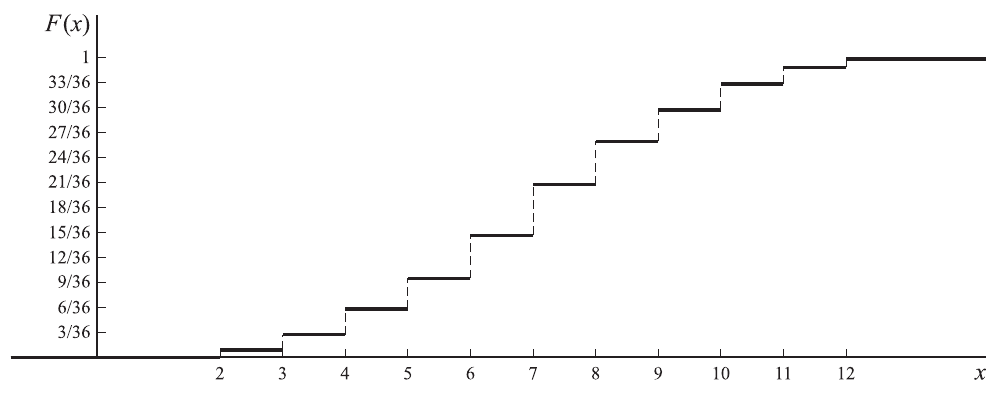
\includegraphics[width=10cm,keepaspectratio=true]{./pe/pands0206.png}
	% pands0206.png: 0x0 pixel, 300dpi, 0.00x0.00 cm, bb=
	\label{fig:2.6.2}
\end{figure}

\begin{ejemplo}
	\label{exmp:2.6.7}
	\begin{enumerate}
		\item Find the distribution function $F(x)$ for the random variable of Solved Problem \ref{exmp:2.6.4};
		\item graph this distribution function.
	\end{enumerate}
\end{ejemplo}

\begin{figure}
	\centering
	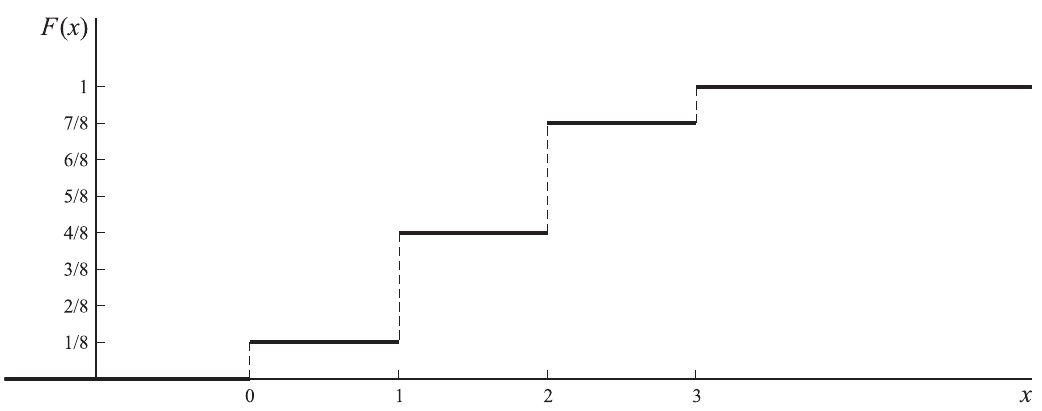
\includegraphics[width=10cm,keepaspectratio=true]{./pe/pands0207.png}
	% pands0206.png: 0x0 pixel, 300dpi, 0.00x0.00 cm, bb=
	\label{fig:2.6.3}
\end{figure}

\subsection{Expected Value and Variance for Discrete Random Variables}

\subsubsection{Expected Value of a Discrete Random Variable}
For a discrete random variable $X$ with probability mass function $f(x) = P(X=x)$ and support $S_X = \set{x_1, x_2, \dots, x_n, \dots}$, the \emph{mathematical expectation} or \emph{expected value} is defined as the weighted average of its possible values:
\begin{align}
	\label{eq:esperanza_discreta}
	\mu = \mathbb{E}[X] = \sum_{x \in S_X} x f(x).
\end{align}
The expected value exists if and only if the sum converges absolutely ($\sum_{x \in S_X} |x| f(x) < \infty$). Physically, the expected value represents the center of mass of the probability distribution on the number line.

\subsubsection{Discrete Variance and Standard Deviation}
The \emph{variance} of a discrete random variable measures the mean squared dispersion about the expectation $\mu$:
\begin{align}
	\label{eq:varianza_discreta}
	\sigma^2 = \s^2 = \Var(X) = \mathbb{E}\left[(X - \mu)^2\right] = \sum_{x \in S_X} (x - \mu)^2 f(x).
\end{align}
By linearity of the expectation operator, the shortcut computational formula for the variance is:
\begin{align}
	\label{eq:varianza_formula_corta}
	\Var(X) = \mathbb{E}[X^2] - (\mathbb{E}[X])^2 = \sum_{x \in S_X} x^2 f(x) - \mu^2,
\end{align}
where $\mathbb{E}[X^2]$ is the second raw moment of the variable. The standard deviation is the square root of the variance: $\sigma = \sqrt{\Var(X)}$.
